\documentclass[a4paper]{scrartcl}

\usepackage[
    fancytheorems, 
    fancyproofs, 
    noindent, 
]{adam}

\usepackage{tikz}
\usepackage{cancel}

\title{Methods}
\author{Adam Kelly (\texttt{ak2316@cam.ac.uk})}
\date{\today}

\allowdisplaybreaks

\begin{document}

\maketitle

% Our goal is to setup a framework to solve PDEs in many contexts.
% 

% This is a short description of the course. It should give a little flavour of what the course is about, and what will be roughly covered in the notes.

This article constitutes my notes for the `Methods' course, held in Michaelmas 2021 at Cambridge. These notes are \emph{not a transcription of the lectures}, and differ significantly in quite a few areas. Still, all lectured material should be covered.



\tableofcontents

% \part{Self-Adjoint ODEs}

\section{Fourier Series}

\subsection{Periodic Functions}

We will begin our study of method and in particular Fourier series by considering some periodic functions.

\begin{definition}[Perioidic]
    A function $f(x)$ is \vocab{periodic} if $f(x + T) = f(x)$ for all $x$, where $T$ is the \vocab{period}. 
\end{definition}

\begin{example}[Simple Harmonic Motion]
    Many physical objects are described by \emph{simple harmonic motion}, with the position given by
    $$
    y = A \sin \omega t.
    $$
    We call $A$ the \vocab{amplitude}, and the period is $T = 2 \pi / \omega$. The \vocab{frequency} is $1/T$.
\end{example}

Fourier series is all about trying to write periodic functions as particular sums of sines and cosines. 
Consider the set of functions
$$
g_n(x) = \cos \frac{n \pi x}{L}, \quad \text{and} \quad h_n(x) = \sin \frac{n \pi x}{L},
$$
where we take $n \in \R^+$.  These functions are periodic on the interval $[0, 2L]$.

You may recall the following set of identities:
\begin{align*}
    \cos A \cos B &= \frac{1}{2}\left(\cos(A - B) + \cos(A + B)\right) \\
    \sin A \sin B &= \frac{1}{2}\left(\cos(A - B) - \cos(A + B)\right) \\
    \sin A \cos B &= \frac{1}{2}\left(\sin(A - B) + \sin(A + B)\right).
\end{align*}
We are going to try and define an inner product on this domain $[0, 2L]$, and using that we will by able to multiply these functions together and talk about their relative orthogonality.

\begin{definition}
    We define the inner product
    $\langle f, g \rangle = \int_0^{2L} f(x) g(x) \dd x$.
\end{definition}

We can then obtain some orthogonality conditions for $h_n$ and $g_n$ with respect to this inner product. We can compute for $n \neq m$
\begin{align*}
    \langle h_n, h_m \rangle &= \int_0^{2L} \sin \frac{n \pi x}{L} \sin \frac{m \pi x}{L} \dd x \\
    &= \frac{1}{2}\int_0^{2L} \left(\cos \frac{(n -m) \pi }{L}x - \cos \frac{(n + m )\pi}{L} x\right) \dd x \\
    &= \frac{1}{2} \frac{L}{\pi}\left[\frac{\sin (n - m) \pi x /L}{n - m} - \frac{\sin (n + m) \pi x /L}{n - m}\right]_0^{2L} \\
    &= 0,
\end{align*}
and for $n = m$
\begin{align*}
    \langle h_n, h_n \rangle &= \int_0^{2L} \sin^2 \frac{n \pi x}{L} \dd x \\
                             &= \int_0^{2L} \frac{1}{2}\left(1 - \cos \frac{2 \pi n x}{L}\right) \dd x \\
                             &= L.
\end{align*}
Hence we obtain the orthogonality condition
$$
\langle h_n, h_m \rangle = \begin{cases}
    L \delta_{mn} &\mbox{if } n, m \neq 0, \\
    0 &\mbox{if } m = 0.
   \end{cases}
$$
Similarly, it's straightforward to check that
$$
\langle g_n, g_m \rangle = \begin{cases}
    L \delta_{mn} &\mbox{if } n, m \neq 0, \\
    2L \delta_{0n} &\mbox{if } m = 0.
   \end{cases}
$$
and
$$
\langle h_n, g_m \rangle = 0.
$$

These orthogonality conditions are important because we are going to use these functions as a complete orthogonal set which spans the space of `well-behaved periodic functions'.


\subsection{Definition of a Fourier Series}

We can express any `well-behaved' periodic function $f(x)$ with period $2L$ as
$$
f(x)=\frac{1}{2} a_{0}+\sum_{n=1}^{\infty} a_{n} \cos \frac{n \pi x}{L}+\sum_{n=1}^{\infty} b_{n} \sin \frac{n \pi x}{L},
$$
where $a_n$, $b_n$ are constants such that the RHS is convergent for all $x$ where $f$ is continuous. At a discontinuity, the Fourier series approaches the midpoint of the upper and lower limits at that point.

Consider taking the inner product $\langle h_n, f\rangle$ and substitute the expression for $f$ above, to get
$$
   \int_0^{2L} \sin \frac{m\pi x}{L} f(x) \dd x = \sum_{n = 1}^{\infty} L b_n \delta_{nm} = Lb_m.
$$
Hence we find that (doing something similar with $g_n$)
\begin{align*}
   b_n &= \frac{1}{L}\int_0^{2L} g(x) \sin \frac{n \pi x}{L} \dd x, \\
    \text{and} \quad a_n &= \frac{1}{L}\int_0^{2L} f(x) \cos \frac{n \pi x}{L} \dd x.
\end{align*}

Now, this expression for $a_n$ includes the case $n = 0$, and says that it is the average value of the function. Also, the range of integration is one period, and we can equivalently integrate over $[-L, L]$ instead of $[0, 2L]$.

\begin{example}[The Sawtooth Wave]
    Consider the function $f(x) = x$ for $-L \leq x \leq L$, with the function being periodic elsewhere.


	\begin{center}
		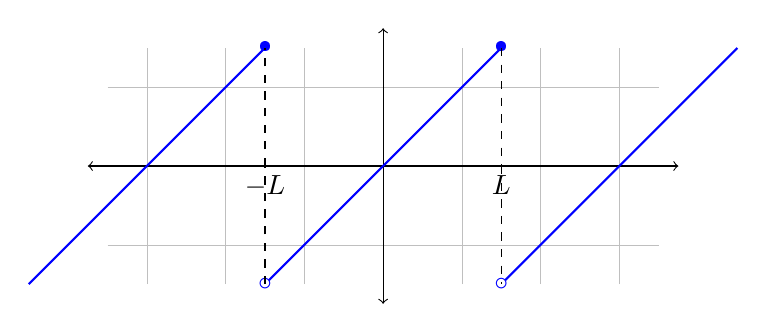
\begin{tikzpicture}
	  \draw[ultra thin,color=lightgray] (-3.5,-1.5) grid (3.5,1.5);   % coordinate grid
	  \draw[<->] (-3.75,0) -- (3.75,0);% node[right] {$x$};   % x-axis
	  \draw[<->] (0,-1.75) -- (0,1.75);% node[above] {$y$};   % y-axis
	
      \draw [thick, samples=100,smooth, color=blue] plot[variable=\t, domain=-4.5:-1.5] ({\t},{\t + 3});
      \draw [thick, samples=100,smooth, color=blue] plot[variable=\t, domain=-1.45:1.5] ({\t},{\t});
      \draw [thick, samples=100,smooth, color=blue] plot[variable=\t, domain=1.55:4.5] ({\t},{\t - 3});

      \node at (-1.5, -1.5) {\color{blue} $\circ$};
	\node at (-1.5, 1.5) {\color{blue} \textbullet};

      \node at (1.5, -1.5) {\color{blue} $\circ$};
	\node at (1.5, 1.5) {\color{blue} \textbullet};

    \draw  [dashed] (1.5, 1.5) -- (1.5, 0) node [below] {$L$};
    \draw [dashed] (1.5, 0) -- (1.5, -1.5);
    \draw  [dashed] (-1.5, -1.5) -- (-1.5, 0) node [below] {$-L$};
    \draw [dashed] (-1.5, 0) -- (-1.5, 1.5);

	\end{tikzpicture}
	\end{center}

    Here we have
    $$
a_n = \frac{1}{L}\int_{-L}^L x \cos \frac{n \pi x}{2} \dd x = 0, \quad \quad \text{(integrating an odd function)}
    $$
    for all $n$, and
    \begin{align*}
        b_n &= \frac{2}{L} \int_0^L x \sin \frac{n \pi x}{L} \dd x   \\
            &= \frac{-2}{n \pi}\left[x \cos \frac{n \pi x}{L}\right]_{0}^{L} + \frac{2}{n \pi} \int_{0}^{h} \cos \frac{n \pi x}{L} \dd x \\
            &= -\frac{2 L}{n \pi} \cos n \pi+\frac{2 L}{(n \pi)^{2}} \cancel{\sin n \pi} \\
            &= \frac{2L}{n \pi} (-1)^{n + 1}.
    \end{align*}
    So the sawtooth Fourier series is 
    $$
    2 L \sum_{n=1}^{\infty} \frac{(-1)^{n+1}}{n \pi} \sin \left(\frac{n \pi x}{L}\right)=\frac{2 L}{\pi}\left[\sin \left(\frac{\pi x}{L}\right)-\frac{1}{2} \sin \left(\frac{2 \pi x}{L}\right)+\frac{1}{3} \sin \left(\frac{3 \pi x}{L}\right) + \cdots\right].
    $$
    which is slowly convergent.

    %L = 1.5
    \begin{center}
    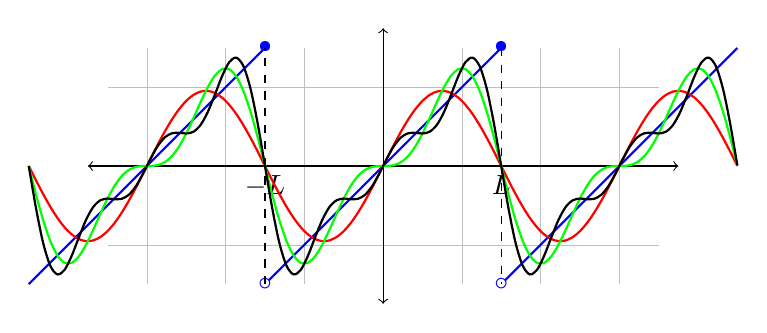
\begin{tikzpicture}
        \draw[ultra thin,color=lightgray] (-3.5,-1.5) grid (3.5,1.5);   % coordinate grid
        \draw[<->] (-3.75,0) -- (3.75,0);% node[right] {$x$};   % x-axis
        \draw[<->] (0,-1.75) -- (0,1.75);% node[above] {$y$};   % y-axis
      
        \draw [thick, samples=100,smooth, color=blue] plot[variable=\t, domain=-4.5:-1.5] ({\t},{\t + 3});
        \draw [thick, samples=100,smooth, color=blue] plot[variable=\t, domain=-1.45:1.5] ({\t},{\t});
        \draw [thick, samples=100,smooth, color=blue] plot[variable=\t, domain=1.55:4.5] ({\t},{\t - 3});
  
        \node at (-1.5, -1.5) {\color{blue} $\circ$};
      \node at (-1.5, 1.5) {\color{blue} \textbullet};
  
        \node at (1.5, -1.5) {\color{blue} $\circ$};
      \node at (1.5, 1.5) {\color{blue} \textbullet};
  
      \draw  [dashed] (1.5, 1.5) -- (1.5, 0) node [below] {$L$};
      \draw [dashed] (1.5, 0) -- (1.5, -1.5);
      \draw  [dashed] (-1.5, -1.5) -- (-1.5, 0) node [below] {$-L$};
      \draw [dashed] (-1.5, 0) -- (-1.5, 1.5);

      % Fourier Series

      \draw [thick, samples=100,smooth, color=red] plot[variable=\t, domain=-4.5:4.5] ({\t},{(2*1.5/pi) * (sin(180 * \t / 1.5))});
      \draw [thick, samples=100,smooth, color=green] plot[variable=\t, domain=-4.5:4.5] ({\t},{(2*1.5/pi) * (sin(180 * \t / 1.5) - 0.5 * sin(2 * 180 * \t / 1.5))});
      \draw [thick, samples=100,smooth, color=black] plot[variable=\t, domain=-4.5:4.5] ({\t},{(2*1.5/pi) * (sin(180 * \t / 1.5) - 0.5 * sin(2 * 180 * \t / 1.5) + (1/3) * sin(3 * 180 * \t / 1.5))});
      
      \end{tikzpicture}
      \end{center}
\end{example}
% \begin{proposition}[Properties of $\sin$ and $\cos$]
    
% \end{proposition}


\end{document}
